\documentclass[tikz,border=3pt]{standalone}
\usepackage[utf8]{inputenc}
\usepackage[T1]{fontenc}
\usepackage{lmodern}
\renewcommand{\familydefault}{\sfdefault}
\usepackage{sansmath}\sansmath
\usepackage{chemfig}
\usepackage{pgfplots}\pgfplotsset{compat=1.18,/pgf/number format/use comma,/pgf/number format/1000 sep={.}}
\usetikzlibrary{arrows.meta,calc,positioning,decorations.pathmorphing,patterns}
% paleta del sitio
\definecolor{nar}{HTML}{E8680C}\definecolor{narc}{HTML}{FFB35C}\definecolor{hielo}{HTML}{FFF3E8}
\definecolor{tinta}{HTML}{1D1D1F}\definecolor{gris}{HTML}{6E6E73}\definecolor{lila}{HTML}{7C5CF0}
\definecolor{azul}{HTML}{2F6FD6}\definecolor{menta}{HTML}{17A673}\definecolor{coral}{HTML}{E8342A}
\begin{document}
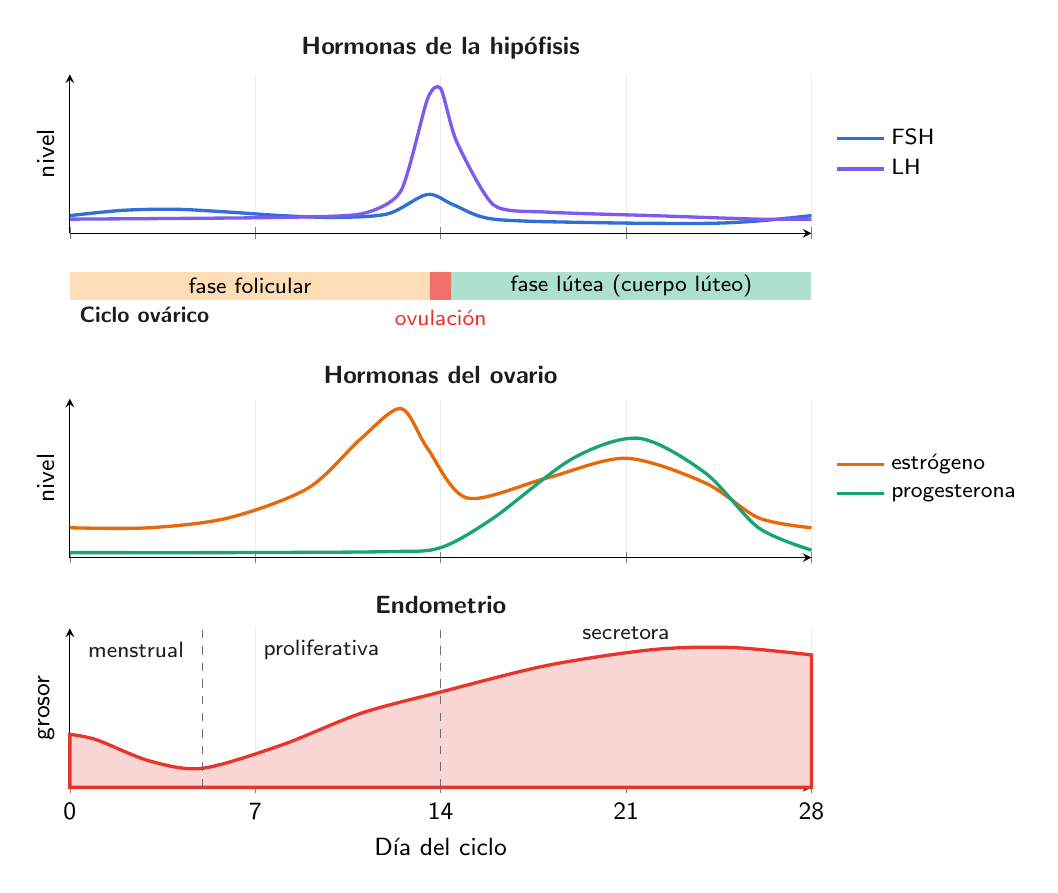
\begin{tikzpicture}[font=\small]
\pgfplotsset{panel/.style={width=11cm,height=3.6cm,xmin=0,xmax=28,ymin=0,axis lines=left,ytick=\empty,xtick={0,7,14,21,28},
 xticklabels={},grid=major,grid style={gray!15},title style={font=\small\bfseries,text=tinta,yshift=-4pt},legend cell align=left,legend style={draw=none,fill=none,font=\footnotesize,at={(1.02,0.5)},anchor=west},clip=false}}
% hipofisis
\begin{axis}[panel,name=a,ymax=45,title={Hormonas de la hipófisis},ylabel={nivel}]
\addplot[azul,very thick,smooth] coordinates {(0,5)(2,6.5)(4,6.8)(6,6)(8,5)(10,4.5)(12,5.5)(13.5,11)(14.5,8)(16,4)(20,3)(24,2.8)(26,3.5)(28,5)};
\addlegendentry{FSH}
\addplot[lila,very thick,smooth,tension=0.4] coordinates {(0,4)(4,4.2)(8,4.5)(11,5.5)(12.5,12)(13.5,38)(14,41)(14.6,26)(16,8)(18,6)(22,5)(26,4)(28,4)};
\addlegendentry{LH}
\fill[narc!45] (axis cs:0,-19) rectangle (axis cs:13.6,-11); \node[font=\footnotesize] at (axis cs:6.8,-15) {fase folicular};
\fill[coral!70] (axis cs:13.6,-19) rectangle (axis cs:14.4,-11);
\fill[menta!35] (axis cs:14.4,-19) rectangle (axis cs:28,-11); \node[font=\footnotesize] at (axis cs:21.2,-15) {fase lútea (cuerpo lúteo)};
\node[font=\footnotesize\bfseries,text=tinta,anchor=west] at (axis cs:0,-23) {Ciclo ovárico};
\node[font=\footnotesize,text=coral,anchor=north] at (axis cs:14,-19) {ovulación};
\end{axis}
% hormonas ovario
\begin{axis}[panel,name=b,at={(a.south west)},anchor=north west,yshift=-2.1cm,ymax=32,title={Hormonas del ovario},ylabel={nivel}]
\addplot[nar,very thick,smooth] coordinates {(0,6)(3,6)(6,8)(9,14)(11,24)(12.5,30)(13.5,22)(15,12)(18,16)(21,20)(24,15)(26,8)(28,6)};
\addlegendentry{estrógeno}
\addplot[menta,very thick,smooth] coordinates {(0,1)(6,1)(12,1.2)(14,2)(16,8)(19,20)(21.5,24)(24,17)(26,6)(28,1.5)};
\addlegendentry{progesterona}
\end{axis}
% endometrio
\begin{axis}[panel,name=c,at={(b.south west)},anchor=north west,yshift=-0.9cm,ymax=15,title={Endometrio},ylabel={grosor},xticklabels={0,7,14,21,28},xlabel={Día del ciclo}]
\addplot[coral,very thick,smooth,fill=coral!20] coordinates {(0,5)(1,4.5)(3,2.5)(5,1.8)(8,4)(11,7)(14,9)(18,11.5)(22,13)(25,13.2)(28,12.5)} \closedcycle;
\node[font=\footnotesize,text=tinta] at (axis cs:2.5,13) {menstrual};
\node[font=\footnotesize,text=tinta] at (axis cs:9.5,13) {proliferativa};
\node[font=\footnotesize,text=tinta] at (axis cs:21,14.6) {secretora};
\draw[gris,dashed] (axis cs:5,0) -- (axis cs:5,15) (axis cs:14,0) -- (axis cs:14,15);
\end{axis}
\end{tikzpicture}
\end{document}
